%%%% ijcai19.tex

\typeout{Probabilistic Robust Multi-Agent Path Finding}


\newcommand{\tuple}[1]{\ensuremath{\left \langle #1 \right \rangle }}

% These are the instructions for authors for IJCAI-19.

\newcommand{\qed}{\hfill\ensuremath{\blacksquare}}
\newcommand{\astar}{A$^*$}
\newcommand{\SAS}{SAS$^+$}
\newcommand{\wastar}{WA$^*$}
\newcommand{\arastar}{ARA$^*$}
\newcommand{\open}{\textsc{Open}}
\newcommand{\closed}{\textsc{Closed}}
\newcommand{\cmfp}{conformant model-free planning}
\newcommand{\eff}{\textit{eff}}
\newcommand{\pre}{\textit{pre}}
\newcommand{\solvable}{\textit{S}}
\newcommand{\plannable}{\textit{P}}
\newcommand{\true}{\textit{T}}
\newcommand{\false}{\textit{$\bot$}}


% This is for the agmin


\documentclass{article}
\pdfpagewidth=8.5in
\pdfpageheight=11in
% The file ijcai19.sty is NOT the same than previous years'
\usepackage{ijcai19}

% Use the postscript times font!
\usepackage{times}
\usepackage{soul}
\usepackage{url}
\usepackage[hidelinks]{hyperref}
\usepackage[utf8]{inputenc}
\usepackage[small]{caption}
\usepackage{graphicx}
\usepackage{amsmath}
\usepackage{booktabs}

\usepackage{float}

%\usepackage{algorithm}
%\usepackage{algorithmic}
\urlstyle{same}

\usepackage{algorithmic}


\usepackage[usenames,dvipsnames]{xcolor}
\usepackage[ruled,vlined,linesnumbered]{algorithm2e}
\usepackage{amsmath}
\usepackage{amsthm}
\usepackage{url}
\usepackage{multirow}

\usepackage{xspace}
\newcommand{\krmapf}{$k$R-MAPF\xspace}
\newcommand{\krcbs}{$k$R-CBS\xspace}
\newcommand{\ikrcbs}{I-$k$R-CBS\xspace}
\newcommand{\prcbs}{$p$R-CBS\xspace}
\newcommand{\iprcbs}{I-$p$R-CBS\xspace}
\newcommand{\prmapf}{$p$R-MAPF\xspace}



%
% Add comments in the text
%
\newboolean{showcomments}
\setboolean{showcomments}{true}
%\setboolean{showcomments}{false}

\ifthenelse{\boolean{showcomments}}
  {\newcommand{\nb}[3]{
  {\color{#2}\small\fbox{\bfseries\sffamily\scriptsize#1}}
  {\color{#2}\sffamily\small$\triangleright~$\textit{\small #3}$~\triangleleft$}
  }
  }
  {\newcommand{\nb}[3]{}
  }

\newcommand\Dor[1]{\nb{\textbf{Dor:}}{red}{#1}}
\newcommand\Roni[1]{\nb{\textbf{Roni:}}{orange}{#1}}
\newcommand\Ariel[1]{\nb{\textbf{Ariel:}}{cyan}{#1}}



\newcommand{\inlinecite}[1]{\citeauthor{#1} \shortcite{#1}}

% the following package is optional:
%\usepackage{latexsym} 

% Following comment is from ijcai97-submit.tex:
% The preparation of these files was supported by Schlumberger Palo Alto
% Research, AT\&T Bell Laboratories, and Morgan Kaufmann Publishers.
% Shirley Jowell, of Morgan Kaufmann Publishers, and Peter F.
% Patel-Schneider, of AT\&T Bell Laboratories collaborated on their
% preparation.

% These instructions can be modified and used in other conferences as long
% as credit to the authors and supporting agencies is retained, this notice
% is not changed, and further modification or reuse is not restricted.
% Neither Shirley Jowell nor Peter F. Patel-Schneider can be listed as
% contacts for providing assistance without their prior permission.

% To use for other conferences, change references to files and the
% conference appropriate and use other authors, contacts, publishers, and
% organizations.
% Also change the deadline and address for returning papers and the length and
% page charge instructions.
% Put where the files are available in the appropriate places.

\title{Probabilistic Robust Multi-Agent Path Finding}

\newcommand{\OPEN} {{\textsc{Open}}}

\newtheorem{definition}{Definition}
\newtheorem{lemma}{Lemma}
\newtheorem{theorem}{Theorem}
\newcommand{\ignore}[1]{}

% Single author syntax
%\author{IJCAI Submission \#1509
%}

% Multiple author syntax (remove the single-author syntax above and the \iffalse ... \fi here)
% Check the ijcai19-multiauthor.tex file for detailed instructions

\author{
Dor Atzmon$^1$
\and
Ariel Felner$^1$\and
Roni Stern$^1$
\affiliations
$^1$Ben Gurion University of the Negev
\emails
dorat@post.bgu.ac.il,
felner@bgu.ac.il,
sternron@post.bgu.ac.il
}


\begin{document}

\maketitle

% No abstract!
\iffalse
% -----------------   ABSTRACT    -------------------------
\begin{abstract}

In a multi-agent path-finding (MAPF) problem, the task is to find a plan for moving a set of agents from their initial locations to their goals without collisions.  Following this plan, however, may not be possible due to unexpected events that delay some of the agents. Guaranteeing that collisions will never occur may be impossible. An important task is to find a plan that is very likely to succeed, even though unexpected delays may occur. We propose an algorithm for finding a plan in which the probability that no collisions will occur is at least a given parameter $p$ ($p$-robust plan).
We show that finding an optimal $p$-robust plan is significantly more difficult than finding an optimal standard plan. As a practical solution, we propose a greedy algorithm based on the Conflict-Based Search framework. 
Our experiments show that it finds $p$-robust plans with a cost that is relatively close to the optimal cost of the standard, non-robust plans.
\end{abstract}
\fi

% -----------------   Introduction    --------------------------
\section{Introduction and Definitions}
The {\em Multi-Agent Path Finding} (MAPF) problem is defined by a graph $G=(V,E)$ and a set of agents $a_1 \dots a_n$. At each time step, an agent can either {\em move} to an adjacent location or {\em wait} in its current location. The task is to find a plan $\pi_i$ for each agent $a_i$ that moves it from its start location $s_i \in V$ to its goal location $g_i \in V$ such that agents do not {\em conflict}, i.e., occupy the same location at the same time. 

In practice, unexpected events may delay some of the agents, preventing them from following their plans. Thus, it is often desirable to generate a {\em robust plan} that can withstand such delays. Recently, a form of robustness called \emph{$k$-robust MAPF} was introduced~\cite{DBLP:conf/socs/AtzmonSFWBZ18}, in which each agent can be delayed up to $k$ times and no collision will occur. 

In some cases, it is possible to estimate the probability that any single delay will occur. By aggregating the probabilities of multiple delays we can estimate the probability that a given conflict will occur. In such cases, solving all conflicts with the same fixed value $k$ may be less reasonable, and we might prefer solving conflicts based on their probabilities to occur. In this paper we explore a new form of robustness, $p$-robust, that considers such additional information. In $p$-robust MAPF (\prmapf) given a probability $p$, we seek a plan that can be executed without any collisions with a probability $\geq p$. 

% Potential conflicts and a conflict occurring
\begin{definition}[Potential Conflict]
A plan $\pi$ has a potential conflict $C=\tuple{a_i,a_j,t}$ iff there exists $\Delta(C)\geq 0$ such that agents $a_i$ and $a_j$ are located in the same location in time steps $t$ and $t+\Delta(C)$, respectively, i.e, when $\pi_i(t) = \pi_j(t+\Delta(C))$.  
\end{definition}

A potential conflict $C=\tuple{a_i,a_j,t}$ 
is said to {\em have occurred} if agent $a_i$ experienced exactly $d_i\geq \Delta(C)$ delays before performing the $t^{th}$ action in $\pi_i$, 
and agent $a_j$ experienced exactly $d_i-\Delta(C)$ delays before performing the $t+\Delta(C)$ action in $\pi_j$. This means the agents will collide  since $\pi_i(t)=\pi_j(t+\Delta(C))$ (they will collide at time $t+d_i$).
 
% Our setting, and the likelihood of a potential conflict to occur
Let $P_0(\pi,p_d)$, or $P_0(\pi)$ in short, be the probability that no potential conflict will occur when following plan $\pi$ with a delay probability of $p_d$. 
A plan $\pi$ is $p$-robust if the probability that no potential conflicts will occur is $\geq p$, i.e., $P_0(\pi)\geq p$.

% ------------------    p -Robust CBS   ------------------------
\section{\texorpdfstring{$p$}--Robust CBS}
 \label{sec:probust-cbs}
 
\prcbs is a CBS-based algorithm \cite{CBSJUR} designed to return $p$-robust plans.  \prcbs{} is unique in how it handles CT nodes, in how it chooses and resolves conflicts, and in how it orders nodes in the high-level Open list. 

% Handling a CT node
{\bf Handling a CT node.} When a CT node $N$ is chosen for expansion, \prcbs{} scans $N.\pi$ for potential conflicts by checking for locations occupied by more than one agent (even in different time steps). Then, $N.\pi$ is sent to a binary verifier that returns whether the plan is $p$-robust (if $P_0(\pi) \geq p$) or not. If the verifier returns TRUE, then the CT node is declared as goal and $\pi$ is returned. If the verifier returns FALSE, it also returns $P_0(\pi)$ as well as a probability $P_{First}(C)$ for each potential conflict $C$. $P_{First}(C)$ provides the probability that while executing $\pi$, conflict $C$ will occur first in time among all potential conflicts. Note that the sum of $P_0$ and all $P_{First}$ probabilities equals 1, because either the execution succeeded ($P_0$) or one of the conflicts have occurred (one of the $P_{First}$). 


% Choosing a conflict to resolve
{\bf Choosing a Conflict to Resolve.} $p$-robust solution may contain many potential conflicts. Thus, we need to resolve a set of conflicts such that the solution will be $p$-robust. \prcbs{} chooses to resolve the conflict with the highest probability of occurring (highest $P_{First}(C)$). This is a greedy approach that has high chances to reach a $p$-robust plan quickly, as it has the highest potential to increase $P_0$ in its children. 

% Resolving a conflict
{\bf Resolving a Conflict.} Let $C=\tuple{a_i,a_j,t}$ be the chosen potential conflict in a non-goal node $N$. To resolve $C$, we add the range constraints
$\tuple{a_i, \pi_i(t), [t, t+\Delta(C)]}$ and $\tuple{a_j, \pi_j(t+\Delta(C)), [t, t+\Delta(C)]}$ to $a_i$ and $a_j$, respectively. This assures that these agents will not both be at the conflicting location in the time frame $[t,t+\Delta(C)]$.

% Choosing CT Nodes
{\bf Choosing CT Nodes.} In this paper we focused on finding a $p$-robust plan as fast as possible. Therefore, we implemented a greedy approach that chooses to expand the node with highest $P_0$ value. Then,  When a CT node with $P_0\geq p$ is found by a verifier, that node is returned as a goal and the search halts. 


% Figure - pR-CBS Example
\begin{figure}[t]
	\centering
	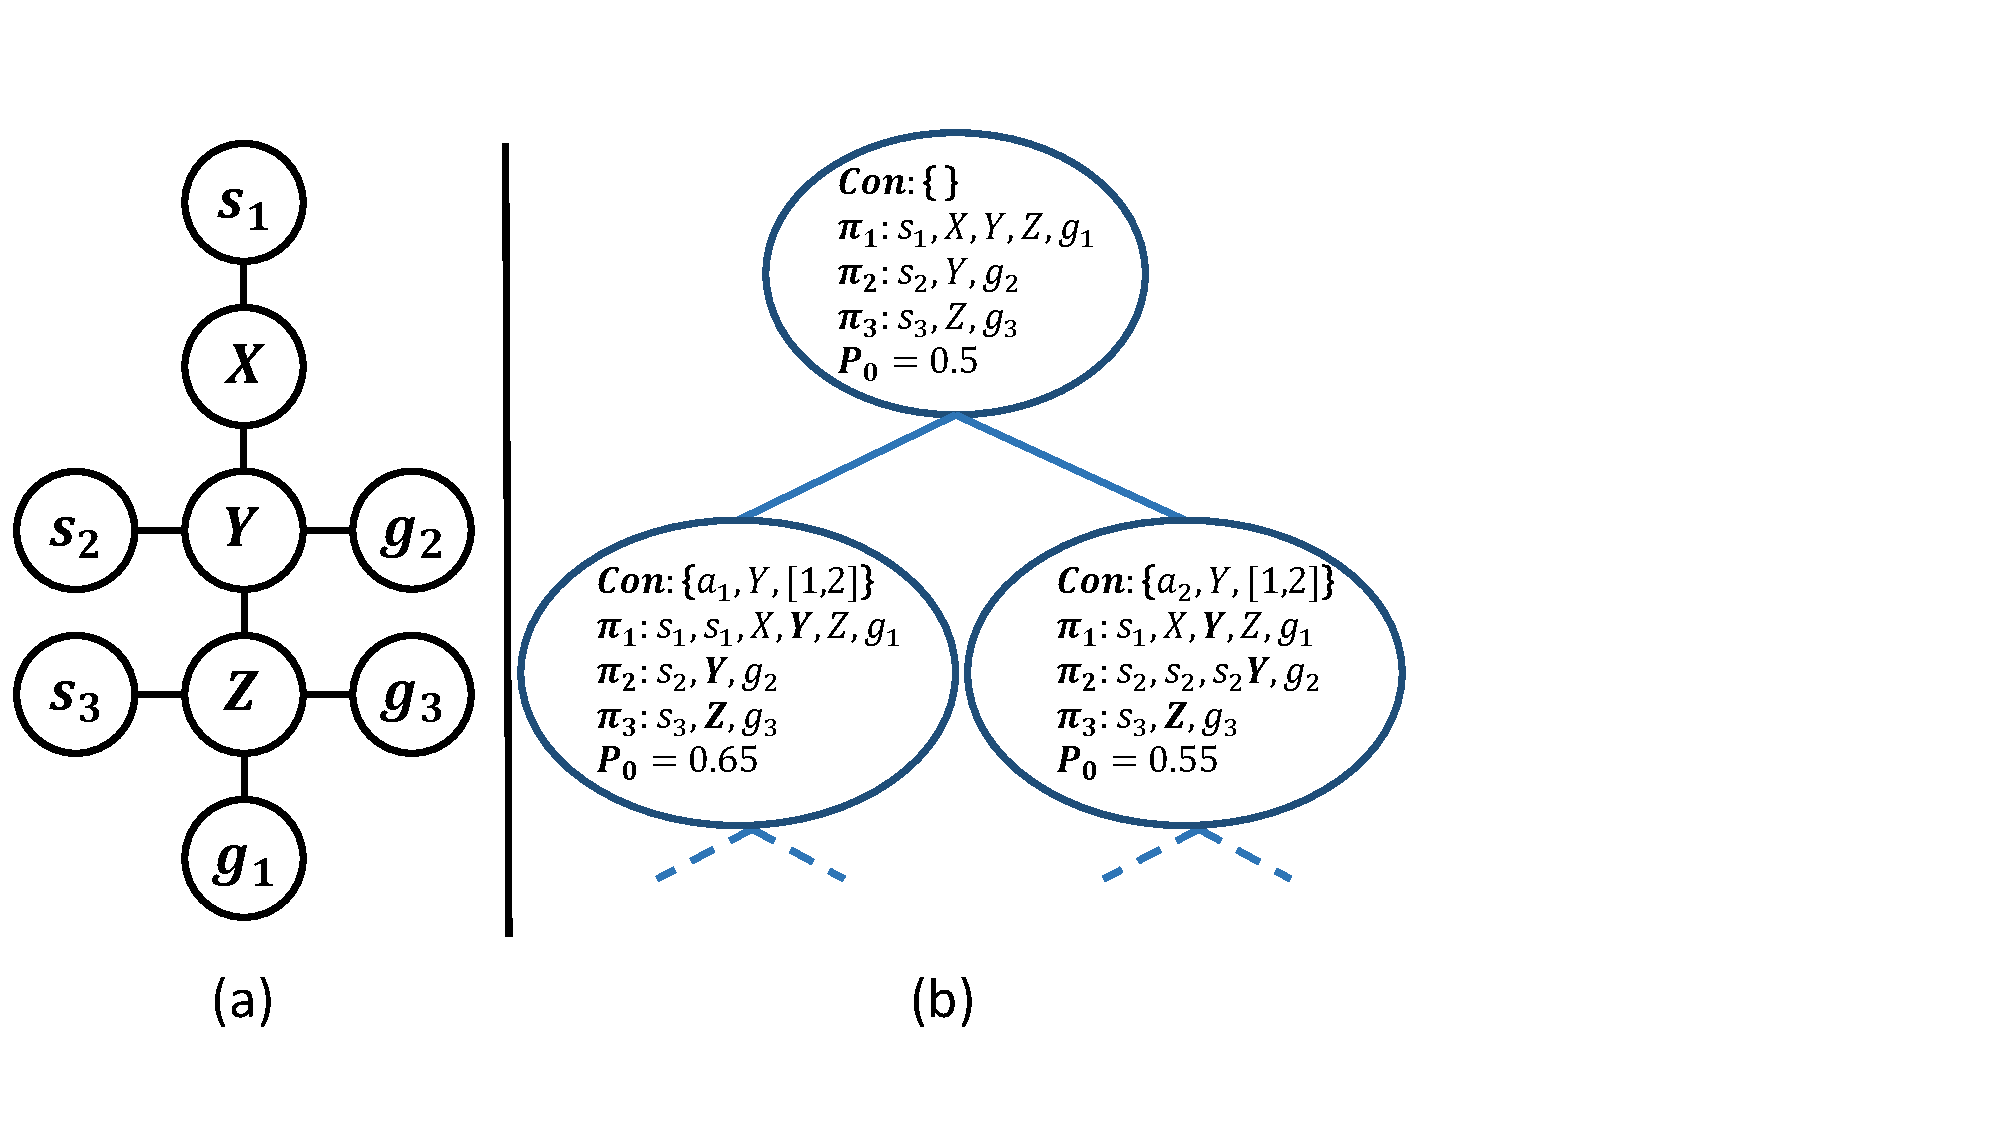
\includegraphics[width=0.7\columnwidth]{Pics/cropped_probust_example.pdf}
	%    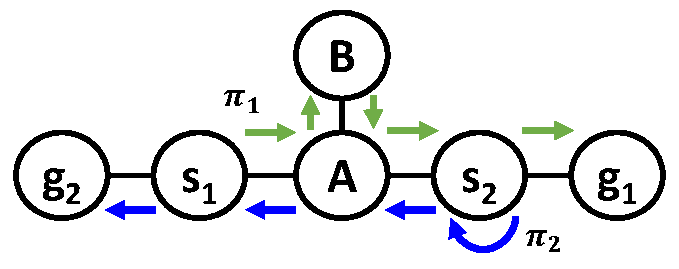
\includegraphics[width=0.9\columnwidth]{lazy-incomplete_cropped.pdf}
	\caption{Example \prcbs{}}
	\vspace{-0.3cm}
	\label{fig:conflicts_example}%\vspace{-0.3cm}
\end{figure}

% Example
{\bf Example.} Figure~\ref{fig:conflicts_example}(a) shows an example of running \prcbs{}. Each of the three agents $a_i$ needs to go from $s_i$ to $g_i$. 
There are two potential conflicts in the initial CT node. $C_Y=\{a_2,a_1, 1\}$ (at location $Y$) where $\Delta(C_Y)=1$ and $C_Z=\{a_3,a_1, 1\}$ (at location $Z$) where $\Delta(C_Z)=2$.
Figure~\ref{fig:conflicts_example}(b) illustrates the corresponding CT. Assume that the verifier returned that $P_{First}(C_Y)=0.3$, $P_{First}(C_Z)=0.2$, and $P_0=0.5$. Assuming $p=0.6$, the verifier returns that the root is not a goal node. We split the root by the conflict with the highest $P_{First}$ ($C_Y$). Since $C_Y=\{a_2,a_1, 1\}$ and $\Delta(C_Y)=1$, we resolve $C_Y$ by the set of constraints $\{a_1,Y,[1,2]\}$ and $\{a_2,Y,[1,2]\}$, so that each generates a new CT child node.  We now choose the node with the highest $P_0$, the left node. The verifier determines that node as a goal, and \prcbs{} halts. 


% ------------------   Statistical Verifier   ---------------------
\section{Statistical Verifiers}
\label{sec:stat-verifier}
We describe two verifiers that verify statistically whether $P_0$ is {\em greater than or equal to} the desired robustness ($p$). %The first verifier performs a fixed number of simulations (Fixed Verifier) while the second verifier dynamically performs simulations (Dynamic Verifier).


% Fixed Verifier
{\bf Fixed Verifier.} The fixed verifier is first initialized with the following given parameters: $p$, $p_d$, $s$, and $\alpha$, where $p$ is the desired robustness, $p_d$ is the constant delay probability, $s$ is the number of simulations to be performed, and $1-\alpha$ is the confidence level of the statistical test. Then, a {\em critical value} $c_1$ is calculated by performing a $Z$-test as follows:
\begin{equation}
{  c_1=p+Z_{1-\alpha} \cdot \sqrt{\frac{(1-p) \cdot p}{s}}}
\label{equ:critical}
\end{equation}

$c_1$ is calculated once and used later in every verification to determine whether $P_0 \geq p$ within the confidence level $1-\alpha$.

After \prcbs{} has chosen to expand node $N$, it calls the fixed verifier to verify statistically whether $N$ is a goal node. The verifier executes $s$ simulations of the given plan ($N.\pi$) with delay probability $p_d$. To count collisions during executions we create a table (named $\mathit{occurred}$) that maps a given potential conflict to the number of times it has occurred. We also initialize a parameter: $\mathit{successes}$ that counts the number of executions in which no collision has occurred. During each execution, if a collision has occurred at a potential conflict $C$, the execution halts, and we increment $\mathit{occurred[C]}$ (initialized as $0$). Otherwise, if no collision has occurred, we increment $\mathit{successes}$. When all $s$ simulations ended, it sets $P_0 \gets \mathit{successes}/s$. If $P_0 > c_1$, it returns TRUE. Otherwise, it sets $N.P_0 \gets P_0$. For each conflict $C$ it sets $N.P_{First}(C) \gets \mathit{occurred[C]}/{s}$ and it returns FALSE.

{\bf Dynamic Verifier.} The main drawback of the fixed verifier is that it uses a fixed number of simulations, denoted $s$. However, in some cases $s$ might not be enough and in other cases $s$ is too high. If $P_0 > c_1$ the verify may return true. This may be possible only if $c_1 < 1$. Therefore, we would like to perform enough simulations that will guarantee that $c_1<1$. This is done dynamically with our dynamic verifier described next, that does not use a fixed number of simulations.  

% Initialization
The minimum number of simulation that guarantees that $c_1<1$ can be derived from Equation \ref{equ:critical}, as follows:
\begin{equation}\label{eq2}
    { s \geq \left \lceil {Z_{1-\alpha}}^2 \cdot \frac{p}{1-p} \right \rceil}
\end{equation}



% Verification
After initializing $s$ according to Equation~\ref{eq2}, we perform $s$ simulations. We then consider to add more simulations according to the following protocol. We start by testing if $P_0>c_1$. If the test passes, return TRUE. Otherwise, we might be able to perform more simulations until the test will pass. However, the test might always fail and this will lead to an infinite loop.  To overcome this issue, before increasing $s$ and executing one more simulation, we perform another statistical test that checks whether $P_0<c_2$ where $c_2$ is a new critical value which is calculated as follows:
\begin{equation}
c_2=p-Z_{1-\alpha} \cdot \sqrt{\frac{(1-p) \cdot p}{s}}
\label{equ:critical2}
\end{equation}
If the second test passes, return FALSE. Otherwise, increment $s$, execute one more simulation, and perform these two tests again. The verification phase of the dynamic verifier summarized as follows. (1) Run $s$ simulations and approximate $P_0$. (2) Calculate $c_1$  (Equation~\ref{equ:critical}). (3) If $P_0>c_1$, return TRUE. (4) Calculate $c_2$ (Equation~\ref{equ:critical2}). (5) If $P_0<c_2$, return FALSE. (6) $s \gets s+1$, run one more simulation, and goto step 2.


% ----------------   Experimental Results   ----------------------
\section{Experimental Results}
\label{sec:experiments1}

We experimentally compared the performance of \prcbs{} with different values of robustness $p$ with our two verifiers. In all of the following results $\alpha=0.05$, $p_d=0.2$, and $P_0$ was calculated based on 50 executions of the solution. 

% Results - p comparison
\begin{table}[t]
\centering
\resizebox{0.55\columnwidth}{!}{
\begin{tabular}{|c|r|r|r|}
\hline
\multicolumn{1}{|l|}{} & \multicolumn{1}{c|}{Cost} & \multicolumn{1}{c|}{Time(ms)} & \multicolumn{1}{c|}{$P_0$} \\ \hline
CBS                    & 38.5                      & 9                         & 0.41                       \\
$p=0.6$                  & 41.7                      & 2,553                     & 0.79                       \\
$p=0.7$                  & 43.3                      & 7,620                     & 0.84                       \\
$p=0.8$                  & 44.9                      & 14,915                    & 0.88                       \\
$p=0.9$                  & 50.1                      & 37,501                    & 0.95                       \\ \hline
\end{tabular}}
\caption{Average planning cost, runtime and for CBS and \prcbs{} with different values of $p$,  over 8x8 open grid.}
\label{tab:p-values}
\end{table}

We compared standard CBS and \prcbs{} with the fixed verifier for different values of $p$ (0.6, 0.7, 0.8, and 0.9) and $s=40$, on an 8x8 open grid with 8 randomly allocated agents. Table~\ref{tab:p-values} presents the average cost, planning time (in ms), and $P_0$ for 60 problem instances.
We can see that larger $p$ increases the cost and time but results in less collisions (higher $P_0$). For example, for $p=0.6$ the cost is 41.7, the time is 2,553ms, and $P_0=0.79$, while for $p=0.9$ the cost is 50.1, the time is 37,501, and $P_0=0.95$. The optimal solver (CBS) achieved the lowest cost (38.5) and the fastest planning time (only 9ms) with a tradeoff that many collisions occurred and only 41\% of the executions were collision-free ($P_0$).


% Dynamic Verifier
\begin{table}[t]
\centering
\resizebox{0.85\columnwidth}{!}{
\begin{tabular}{|c|c|c|c|c|}
\hline
\#Simulations & $p=0.80$ & $p=0.8$5 & $p=0.90$ & $p=0.95$ \\ \hline
20            & \textbf{59}     & 0      & 0      & 0      \\
30            & \textbf{59}     & \textbf{59}     & 0      & 0      \\
40            & 58     & 57     & \textbf{57}     & 0      \\
50            & \textbf{59}     & 57     & 55     & 0      \\
60            & 57     & 55     & 55     & 0      \\
80            & \textbf{59}     & 57     & 54     & 51     \\
160           & 58     & 56     & 52     & 49     \\ 
Dynamic       & \textbf{59}     & \textbf{59}     & \textbf{57}     & \textbf{52}     \\ \hline
\end{tabular}}
\caption{Success rate for \prcbs{} out of 60 instances.}
\label{tab:dynamic}
\end{table}

We also compared the fixed verifier (with a different number of simulations) and the dynamic verifier, with $p=0.8,0.85,0.9,$ and $0.95$. 60 instances were generated and we present the number of instances that could be solved within 5 minutes in Table~\ref{tab:dynamic}. As expected, if the number of simulations was too small, the fixed verifier could not solve any instance as a result of the statistic test ($c_1$ was greater than 1). For example, \prcbs{} with $p=0.85$ and 20 simulations did not solve any instance. On the other hand, the dynamic verifier could solve instances for all values of $p$. Moreover, the success rate of the dynamic verifier was at least as the success rate of the fixed verifier that achieved the highest success rate. The quality of solution and running time of the dynamic verifier and the fixed verifier were similar for instances that could be solved by both. The dynamic verifier performs better but it is more complicated. Hence there is a tradeoff.



% ---------------   Conclusions and Future work   -----------------
\section{Conclusions and Future work}

We studied a new form of robustness: $p$-robust, and proposed a greedy CBS-based algorithm for finding a $p$-robust plan with two possible verifiers that have an internal tradeoff. Possible lines of future work, including integrating $p$-robust plans with execution policies, as suggested by Ma et al.~\shortcite{ma2017multiAgent} and a better approximating the real $P_0$ probability.




%-----------------------------------------------
%-----------------------------------------------


%% The file named.bst is a bibliography style file for BibTeX 0.99c
\bibliographystyle{named}
\bibliography{ijcai19}

\end{document}

